90. а) $f(x)=x^2-|2x-1|=\begin{cases} x^2+2x-1,\ x\leqslant\cfrac{1}{2},\\ x^2-2x+1,\ x>\cfrac{1}{2}.\end{cases}$
$$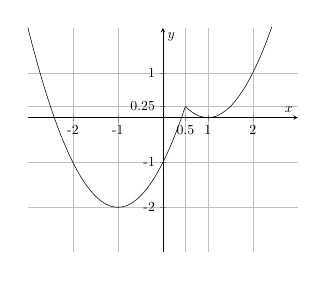
\begin{tikzpicture}[scale=0.5]
\begin{axis}[
    axis lines = middle,
    grid=major,
    legend pos={south west},
    xlabel = {$x$},
    %xlabel style={below right},
    ylabel = {$y$},
    ymin=-3,
    ymax=2,
    xmin=-3,
    xmax=3,
    xtick={-2,-1,0.5, 1,2},
    xticklabels={-2, -1,0.5, 1,2},
    ytick={-2,-1,0.25,1},
    yticklabels={-2,-1,0.25,1},
                  ]
	\addplot[domain=-4:0.5, samples=100, color=black] {(x*x+2*x-1)};
\addplot[domain=0.5:3, samples=100, color=black] {(x*x-2*x+1)};
        %\addplot[domain=2.01:6, samples=100, color=black] {2/(2-x)};
   % \addplot[domain=-3:3, samples=100, color=black] {-x};
     %\addlegendentry{$\text{Рис. 1}$};
\end{axis}
\end{tikzpicture}$$
б) По графику определим количество пересечений функции $f(x)=x^2-|2x-1|$ с горизонтальной прямой $y=a,$ два пересечения будут при $a\in(-2;0)\cup\left(\cfrac{1}{4};+\infty\right).$\\
